\section{五次三维流形高亏格 GW 不变量的结构 (Shuai Guo)}%
\label{sec:Structure of higher-genus GW invariants of the quintic (Shuai Guo)}

\subsection{问题}%
\label{sub:The problem (Guo)}

我们考虑五次三维流形 \(X = X_5 \subset \P^4\)，并问其中包含多少条亏格为 \(g\)、次数为 \(d\) 的曲线。在亏格零时，答案的开头是
\[ 2875, \qquad 609250, \qquad 317206375, \qquad \ldots \]

由于 \(X\) 是 Calabi-Yau 流形，模空间 \(\Mbar_{g,n}(X,\beta)\) 的虚拟维数为零，而弦方程给出 \(\ab<\1, \gamma_2, \ldots, \gamma_n>_{g,n,\beta} = 0\)，除非 \((g,n,\beta) = (0,3,0)\)。因此我们定义基本不变量为
\[ N_{g,\beta} \coloneqq \ab<>_{g,0,\beta} = \int_{[\Mbar_g(X,\beta)]^{\vir}} 1 \]
并将其组装成生成级数
\[ F_g(Q) \coloneqq \sum_{\beta \text{ effective}} N_{g,\beta}Q^{\beta}. \]

不变量 \(N_{g,\beta}\) 是有理数，而我们真正想要的整数是 BPS 不变量 \(n_{g,\beta}\)。它们由正次数部分 \(F_g^+\) 通过多重覆盖变换定义：
\[ \sum_{g \geq 0} F_g^+(Q)\lambda^{2g-2} = \sum_{\substack{g \geq 0 \\ \beta > 0}} n_{g,\beta} \sum_{k \geq 1} \frac{1}{k} \ab(2 \sin \frac{k\lambda}{2})^{2g-2}Q^{k\beta}. \]
注意只有 \(n_{g,\beta}\) 被期望为整数，而上面列出的数是 \(n_{0,d}\)。

\begin{table}[htpb]
    \centering
    \caption{五次三维流形的前几个 BPS 不变量 \(n_{g,d}\)}
    \label{tab:quinticbps}
    \begin{tabular}{crrrrr}
        \toprule
        \(g\) & \(d=1\) & \(d=2\) & \(d=3\) & \(d=4\) & \(d=5\) \\
        \midrule
        0 & 2875 & 609250 & 317206375 & 242467530000 & 229305888887625 \\
        1 & 0 & 0 & 609250 & 3721431625 & 12129909700200 \\
        2 & 0 & 0 & 0 & 534750 & 75478987900 \\
        3 & 0 & 0 & 0 & 8625 & \(-15663750\) \\
        4 & 0 & 0 & 0 & 0 & 49250 \\
        5 & 0 & 0 & 0 & 0 & 1100 \\
        6 & 0 & 0 & 0 & 0 & 10 \\
        7 & 0 & 0 & 0 & 0 & 0 \\
        \bottomrule
    \end{tabular}
\end{table}

我们看到~\Cref{tab:quinticbps} 的每一列最终都变为零。这就是 Castelnuovo 界，对于五次三维流形它断言当 \(g > \frac{d^2+5d+10}{10}\) 时 \(n_{g,d} = 0\)，由 Liu--Ruan~\cite{LiuRuanCastelnuovo} 证明。表中元素的整性即 Gopakumar-Vafa 猜想，由 Ionel--Parker~\cite{IonelParker2018} 证明。

在亏格零时，Candelas-de la Ossa-Green-Parkes 利用镜像上的周期积分计算了 \(F_0\)，我们已在~\Cref{sub:Enumerative mirror symmetry in genus zero} 中讨论过。在高亏格时，Bershadsky-Cecotti-Ooguri-Vafa 给出了一个递推，它由 \(h < g\) 的 \(F_h\) 生成 \(F_g\)，只差有限多个未知常数。我们的目标是解释 log GLSM 如何确定这一不确定性。

\subsection{亏格零与 B-模型的多项式结构}%
\label{sub:Genus zero and the polynomial structure of the B-model}

回顾~\Cref{sub:Enumerative mirror symmetry in genus zero}，对于五次三维流形我们考虑 \(I\)-函数
\[
    I(q,z) = z\sum_{d \geq 0} q^{H/z+d} \frac{\prod_{m=1}^{5d}(5H+mz)}{\prod_{m=1}^d (H+mz)^5} = I_0 z + I_1 H + I_2 \frac{H^2}{z} + I_3 \frac{H^3}{z^2},
\]
其分量被 Picard-Fuchs 算子零化：
\[ D^4 - 5q(5D+1)(5D+2)(5D+3)(5D+4), \qquad D = q \odv{}{q}. \]
若记 \(J_k = I_k/I_0\) 且 \(\frac{I_1}{I_0} = \log q + \tau(q)\)，于是 \(Q = e^{I_1/I_0} = qe^{\tau(q)} = q + O(q^2)\)，则亏格零镜像定理断言
\[ F_0(Q) = \frac{5}{2}\ab(J_1 J_2 - J_3). \]

为了我们的目的，把五次三维流形的公式放在一般的镜像对称图像中有益。设 \(\mc{X} = \ab\{(X,\omega)\}\) 为一族 Calabi-Yau 三维流形，K\"ahler 模为 \(\mc{M} \ni Q = e^{2\pi i \omega}\)，设 \(\mc{X}^{\vee} = \ab\{(X^{\vee},J)\}\) 为镜像族，复模为 \(\mc{M}^{\vee} \ni q\)。Picard-Fuchs 方程的解是 \(X^{\vee}\) 上的周期，组装成
\[ I(z) = zI_0\varphi_0 + I_1 + I_2 z^{-1} + I_3 z^{-2}, \]
它位于 \(z\varphi_0, \varphi_{\alpha}, \varphi^{\alpha}z^{-1}, \varphi^0 z^{-2}\) 的张成空间中。这里 \(I_1 = \sum_{\alpha} I_1^{\alpha}\varphi_{\alpha}\)，\(I_2 = \sum_{\alpha} I_{2,\alpha}\varphi^{\alpha}\)，\(I_3 = I_{3,0}\varphi^0\)，镜像映射仍为 \(Q = e^{I_1/I_0} = qe^{\tau(q)}\)。

我们将使用五次三维流形复模直线上的三个特殊点：大复结构点 \(q=0\)、conifold 点 \(q = 5^{-5}\)（此处一个周期消失）、以及 orbifold（或 Landau-Ginzburg）点 \(q = \infty\)。镜像映射在 \(q=0\) 处定义，其展开给出 Gromov-Witten 不变量，而在高亏格时我们将在另外两点处施加边界条件。

我们现在用三点函数重述镜像定理。取 \(\mc{M}^{\vee}\) 上的局部坐标 \(q_i\)，设 \(\ab\{\phi_i\}\) 为 A 边上对应的基，并定义
\[ C^A_{ijk}(Q) \coloneqq I_0^2 \ab<\phi_i, \phi_j, \phi_k>^X_{0,3}, \qquad C^B_{ijk}(q) \coloneqq \int_{X^{\vee}} \partial_i \partial_j \partial_k \Omega \wedge \Omega. \]

\begin{thm}[Mirror theorem {\cite{Givental1998,LLY1997}}]
    我们有 \(C^A_{ijk}(Q(q)) = C^B_{ijk}(q)\)。而且 \(C^B_{ijk} \in \Delta^{-1}\Q[q]\)，因此它是 \(\mc{M}^{\vee}\) 上的整体亚纯函数，仅沿判别式有极点。
\end{thm}

特别地，在乘以正确次幂的 \(I_0\) 并应用镜像映射后，亏格零生成函数变为 \(q\) 的有理函数，仅沿判别式有极点。因此，它由有限多个系数决定。

\begin{exm}
    对于超平面基下的五次三维流形，
    \[ C_{111} = \frac{5}{1-5^5 q}. \]
\end{exm}

\begin{exm}
    对于 \(X = X_{3,3} \subset \P^2 \times \P^2\)，Yukawa 耦合为
    \begin{align*}
        C_{111} &= \frac{3^4 q_1 (2+3^3q_1+3^3q_2)}{\Delta}, & C_{222} &= \frac{3^4 q_2(2+3^3q_1+3^3q_2)}{\Delta}, \\
        C_{112} &= \frac{(1-3^3q_1-3^3q_2)(1+2\cdot 3^3 q_1 - 3^3 q_2)}{\Delta}, \\
        C_{122} &= \frac{(1-3^3q_1-3^3q_2)(1-3^3q_1+2\cdot3^3q_2)}{\Delta},
    \end{align*}
    其中
    \[ \Delta = 1 - 3\cdot3^3(q_1+q_2) + 3\cdot3^6(q_1^2 - 7q_1q_2+q_2^2) - 3^9(q_1+q_2)^3. \]
\end{exm}

在高亏格时，我们期望归一化势 \(f^A_{g,i}\) 满足
\[ f^A_{g,i}(Q(q)) = f^B_{g,i}(q) \in \Delta^{-(2g-2+n)}\Q[q], \]
其中右端由图的求和计算。

\subsection{BCOV 费曼规则}%
\label{sub:The BCOV Feynman rule}

B 模型 Feynman 规则与全纯反常方程源自~\cite{BCOV1994}。对于五次三维流形，Chang--Guo--Li 在~\cite{CGL2021} 中证明多项式性，在~\cite{CGL2026} 中证明 Feynman 规则。

我们现在把 BCOV 递推讨论为 Feynman 规则。它来自如~\Cref{sub:Operator formalism and geometric quantization} 中辛变换量子化的有限维模型。设 \(\mc{H} = \mc{H}^- \oplus \mc{H}^+ \subset \mc{H}_{\infty}\) 为辛空间，其中 \(d+1 = \dim \mc{H}^+ = \dim \mc{H}^-\)，并设
\[ R = \begin{pmatrix} A & B \\ C & D \end{pmatrix} \in \End \mc{H}, \qquad \mc{Q}(\mbf{x},\bp) = (\bp, D^{-1}\mbf{x}) - \frac{1}{2}(\bp, D^{-1}C\bp). \]
给定全势 \(F(\hbar, \mbf{x})\)，我们形式地由 Gauss 积分定义变换后的势
\[ f(\hbar, \mbf{x}) \coloneqq (\wh{R}F)(\hbar,\mbf{x}) = \ln \int e^{\hbar^{-1}(\mc{Q}(\mbf{x},\bp') - \mbf{x}'\bp') + F(\hbar,\mbf{x}')}\d{\mbf{x}'}\d{\bp'}. \]
用 stationary phase 展开即得图的求和。这里，每条边上的传播子由 \(D^{-1}C\) 给出，顶点由 \(F\) 给出。

对于 Calabi-Yau 三维流形，传播子按指标个数记为 \(S^{\varphi\varphi}\)、\(S^{\varphi}\) 和 \(S\)，顶点为归一化的 A 模型关联函数
\[ P^A_{g,n}(Q) = I_0^{2-2g}\ab<\phi_1, \ldots, \phi_n>^X_{g,n}. \]
注意它们与解量子微分方程的算子 \(S_{\tau}(z)\) 无关，后者将在后面出现。

\begin{exm}
    对于亏格二无标记点的五次三维流形，Feynman 规则为
    \begin{align*}
        f_2^B ={}& P_2 + \frac{1}{2}S^{\varphi\varphi}P_{1,1}^2 + \frac{1}{2}S^{\varphi\varphi}P_{1,2} + (S^{\varphi\varphi})^2 P_{1,1} + \frac{1}{8}(S^{\varphi\varphi})^2 P_{0,4} \\
        &+ \frac{1}{8}(S^{\varphi\varphi})^3 + \frac{1}{12}(S^{\varphi\varphi})^3 + \frac{\chi}{24}S^{\varphi}P_{1,1} + \frac{1}{2}\frac{\chi}{24}S^{\varphi}S^{\varphi\varphi} \\
        &+ \frac{1}{2}\frac{\chi}{24}\ab(\frac{\chi}{24}-1)S,
    \end{align*}
    其中 \(\chi = \chi(X_5) = -200\)。这是关于传播子的三次多项式。
\end{exm}

我们可以如~\Cref{sub:R-matrix action} 那样将其理解为稳定图求和。顶点 \(v\) 贡献低亏格关联函数 \(P_{g_v, \on{val}(v)}\)；内边把两个插入与传播子缩并；腿记录剩下的插入。每张图以 \(\frac{1}{\ab|\Aut \Gamma|}\) 加权。和往常一样
\[ g(\Gamma) = h^1(\Gamma) + \sum_v g_v, \qquad 2g_v - 2 + \on{val}(v) > 0, \]
而 \(f_g^B\) 是所有亏格 \(g\) 稳定图贡献之和。

\subsection{全纯反常方程}%
\label{sub:The holomorphic anomaly equation}

我们现在把递推改写为微分方程。B 模型振幅 \(\mc{F}_g(z,\bar{z})\) 不是全纯的，对 \(g \geq 2\) 其非全纯性由下式给出：
\[ \partial_{\bar{i}} \mc{F}_g = \frac{1}{2}\bar{C}_{\bar{i}}^{jk}\ab( D_j D_k \mc{F}_{g-1} + \sum_{r=1}^{g-1} D_j \mc{F}_r D_k \mc{F}_{g-r} ). \]
这里 \(C_{ijk}\) 是 Yukawa 耦合，\(\bar{C}_{\bar{i}}^{jk}\) 由 \(\bar{C}_{\bar{i}\bar{j}\bar{k}}\) 用 Weil-Petersson 度量提升两个指标得到，\(D_j\) 是 Hodge 线丛适当次幂上的协变导数。右端两项对应 \(\Mbar_g\) 的两种边界层：非分离节点与分离节点。因子 \(\frac{1}{2}\) 忘记了两支的排序。

若选取局部的 \(\bar{\partial}\)-原函数
\[ \partial_{\bar{i}}S^{jk} = \bar{C}_{\bar{i}}^{jk}, \qquad \partial_{\bar{i}}S^j = G_{i\bar{\ell}}S^{\ell j}, \qquad \partial_{\bar{i}}S = G_{i\bar{\ell}}S^{\ell}, \]
则模去一个全纯项，反常方程变为多项式型 PDE：
\[ \pdv{\mc{F}_g}{S^{jk}} = \frac{1}{2}\ab( D_jD_k \mc{F}_{g-1} + \sum_{r=1}^{g-1} D_j \mc{F}_r D_k \mc{F}_{g-r} ). \]
这些传播子仅在相差全纯张量的意义下定义，这种自由度即全纯不确定性的来源。

\begin{rmk}
    在我们将用于五次三维流形的单参数归一化变量中，它读作
    \[ -\partial_0 P_g = \frac{1}{2}P_{g-1,2} + \frac{1}{2}\sum_{r=1}^{g-1}P_{r,1}P_{g-r,1}, \qquad -\partial_1 P_g = 0. \]
\end{rmk}

为理解图求和为何满足此方程，注意在无标记势中非全纯生成元只出现在边因子中。因此沿传播子方向求导即挑出一条边并将其切断。两个半边成为所得低亏格顶点上的标记，而协变导数由除子方程对应于这些标记。切断一个圈得到 \(P_{g-1,2}\)，切断一条分离边得到 \(P_{g_1,1}P_{g_2,1}\)。

\begin{rmk}
    为清楚起见，蕴含只沿一个方向成立。BCOV 图规则蕴含反常方程，但反常方程本身并不能决定图规则。要恢复相同的解，还需要传播子约定、低亏格顶点数据和边界条件。
\end{rmk}

若所有低亏格顶点已知，则右端已知，于是可对非全纯生成元积分得到
\[ P_g = P_g^{\mr{particular}} + f_g(Y), \]
其中有限生成给出全纯不确定性
\[ f_g(Y) = P_g|_{A = B_1 = B_2 = B_3 = 0} = \sum_{i=0}^{3g-3}a_{i,g}Y^i, \qquad Y = (1-5^5q)^{-1}. \]
可见反常方程在每个亏格留下 \(3g-2\) 个未知系数。

\begin{rmk}
    对于五次三维流形，零次数据连同 orbifold 正则性去掉了其中 \(\ceil{\frac{3g-3}{5}}+1\) 个自由度，conifold 间隙又给出 \(2g-2\) 个进一步条件，于是
    \[ 3g-2 - \ab(\ceil*{\frac{3g-3}{5}}+1) - (2g-2) = \floor*{\frac{2g-2}{5}} \]
    个参数剩下，成为真正新的有效不变量。这恰是~\Cref{eqn:balancing condition} 预言的 \(\infty\)-顶点未知数的个数，即满足 \(\beta \leq \frac{2g-2}{5}\) 的 \(\beta\) 的个数。
\end{rmk}

于是我们得到物理学家提出的如下猜想算法：BCOV Feynman 规则、在 Landau-Ginzburg 点处的 orbifold 正则性（一-mill 种 LG/CY 对应，对于五次三维流形是 Guo-Ruan-Janda 正在进行的工作）、以及 conifold 间隙条件。对此还可加上 Gopakumar-Vafa 整性和 Castelnuovo 界。

\subsection{四个理论}%
\label{sub:Four theories}

回顾~\Cref{sec:Log GLSM (Qile Chen)}，log GLSM 带有两个虚拟圈。约化圈回到五次三维流形的 Gromov-Witten 理论，而典则等变圈允许取单位根特殊化，它是半单的，因而可用 Givental-Teleman 计算。二部图求和
\[ \Omega^{\mr{GW}}_{g,n} = \sum_{\Gamma \text{ bipartite}} \frac{1}{\ab|\Aut \Gamma|} \ab( \prod_{v \in V_{\infty}(\Gamma)} c^{\mr{eff}}_{g_v,\beta_v}) \Cont^{\mr{can}}_{\Gamma} \]
把前者用后者表出，代价是在 \(\infty\)-顶点处引入有效不变量 \(c^{\mr{eff}}_{g,\beta}\)。把它们换成形式参数 \(\mbf{C} = \ab\{c_{g,\beta}\}\) 即得\textit{扩张的 \(\mbf{C}\)-族}，其顶点数据由亚纯与 rubber log GLSM 理论提供。

我们将考虑以下四种理论。
\begin{itemize}
    \item \textit{\(t\)-扭曲几何理论}设 \(\lambda_i = 0\) 而保留辅助权 \(t\)。它有稳定映射与稳定商两个版本，其中商版本给出下面的亏格二局域化公式。
    \item \textit{形式五次三维流形}，即形式 \(\lambda\)-扭曲理论，设 \(t = 0\) 且 \(\lambda_i = \zeta_5^i \lambda\)。它是半单 CohFT，因而有通用且可计算的 \(R\)-矩阵。
    \item \textit{扩张的 \(\mbf{C}\)-族}在两者之间插值，是同时带有形式顶点与亚纯顶点的二部图所生活的族。
    \item \textit{五次三维流形的 Gromov-Witten 理论}由设 \(\mbf{C} = \mbf{C}^{\mr{eff}}\) 再令 \(\lambda \to 0\) 得到，是我们想要计算的理论。
\end{itemize}

\begin{warn}
    在高亏格时，\(t\)-扭曲稳定商理论的 \(t^0\) 系数不是形式 \(\lambda\)-扭曲理论的 \(\lambda^0\) 系数。
\end{warn}

\subsection{形式五次流形}%
\label{sub:The formal quintic}

形式五次三维流形及其全纯反常方程在~\cite{LhoPandharipande2019} 中研究；与扩张理论的比较在~\cite{GJRstructure} 中发展。

设 \(E = \mc{O}_{\P^4}(5)\)，设 \(\pi \colon \mc{C} \to \Mbar_{g,n}(\P^4,d)\) 为万有曲线。\(t\)-扭曲圈为
\[ e(R\pi_* f^* E \otimes [1]) \cap [\Mbar_{g,n}(\P^4,d)]^{\vir}, \]
其中 \([1]\) 的等变第一陈类为 \(t\)。转而从完全 \((\C^{\times})^5\)-等变圈出发，形式五次三维流形是单位根特殊化
\[ [\Mbar_{g,n}(\P^4,d)]^{\vir,\lambda} \coloneqq \ab( e(R\pi_*f^*E \otimes [1]) \cap [\Mbar_{g,n}(\P^4,d)]^{\vir}_{(\C^{\times})^5})\Big|_{t=0, \; \lambda_i = \zeta_5^i \lambda}, \]
其中 \(\zeta_5 = e^{2\pi i/5}\)。关系 \(H^5 = \lambda^5\) 使量子积在一般处半单，同时保留 \(\lambda\) 作为参数。

状态空间、单位元与配对由下式给出：
\[ \mc{H}_{\lambda} = \Q(\lambda)[H]/(H^5-\lambda^5), \quad \1 = 1, \quad (\gamma_1,\gamma_2)^{\lambda} = \int_{\P^4, (\C^{\times})^5} e(\mc{O}(5))\gamma_1\gamma_2 \Big|_{\lambda_i = \zeta_5^i\lambda}, \]
而 CohFT 类为
\[ \Omega^{\lambda}_{g,n}(\gamma_1, \ldots, \gamma_n) = \sum_{d \geq 0} q^d \rho_* \ab( \prod_{i=1}^n \ev_i^*(\gamma_i) \cap [\Mbar_{g,n}(\P^4,d)]^{\vir,\lambda}), \]
其中 \(\rho\) 忘记映射并稳定化定义域。若用 \(\tau(q)H\) 平移，其中 \(\tau(q) = I^{\lambda}_1(q)/I^{\lambda}_0(q)\)，则平移后的理论 \(\Omega^{\lambda,\tau}\) 是半单的。把系数扩到 \(\Q(\zeta_5,\lambda)\) 后，幂等基满足
\[ \omega^{\lambda}_{g,n}(e_{\alpha_1}, \ldots, e_{\alpha_n}) = \sum_{\alpha}\Delta_{\alpha}^{g-1}\prod_i \delta_{\alpha,\alpha_i}. \]
于是~\Cref{thm:teleman} 给出
\[ \Omega^{\lambda,\tau}_{g,n} = \sum_{\Gamma \in G_{g,n}} \frac{1}{\ab|\Aut\Gamma|}\iota_* \Cont_{\Gamma} \]
及~\Cref{sub:R-matrix action} 中的装饰。带 \(\gamma\) 的腿得 \(R^{-1}(\bar{\psi})\gamma\)，边得
\[ V_R(z_1,z_2) = \frac{\sum_{\alpha} e_{\alpha}\otimes e^{\alpha} - \sum_{\alpha} R^{-1}(z_1)e_{\alpha} \otimes R^{-1}(z_2)e^{\alpha}}{z_1+z_2}, \]
顶点得拓扑场论 \(\omega\)，遗忘标记处缺失的保单位部分由 \(T(z) = z(\1 - R^{-1}(z)\1)\) 插入。

\begin{rmk}
    可见边因子没有极点。置 \(z_2 = -z_1\) 并用形如 \(R^{-1}(z) = R^*(-z)\) 的辛条件，分子消失。因此它被 \(z_1+z_2\) 整除，\(V_R\) 是两个余切线变量的幂级数。\(z_1^p z_2^q\) 的系数是放在带 \(\bar{\psi}_1^p \bar{\psi}_2^q\) 的节点处的类，把它与两边相邻的拓扑场论张量缩并即把两支粘合。
\end{rmk}

\subsection{如何计算 \(R\)-矩阵}%
\label{sub:How to compute the R-matrix (Guo)}

要计算 \(R\)-矩阵，我们从形式等变 \(I\)-函数出发：
\[ I^{\lambda}(q,z) = z\sum_{d\geq0}q^d \frac{\prod_{m=1}^{5d}(5H+mz)}{\prod_{m=1}^d ((H+mz)^5 - \lambda^5)} = zI_0 + I_1^{\lambda}H + z^{-1}I_2^{\lambda}H^2 + \cdots. \]
到 \(H\) 为止的系数与 \(\lambda\) 无关，所以 \(I_1^{\lambda} = I_1 - I_0 \log q\)，镜像平移 \(\tau(q) = I_1^{\lambda}(q)/I_0(q)\) 不含对数。设
\[ D = q\odv{}{q}, \qquad Y = (1-5^5q)^{-1}, \qquad L = Y^{1/5} \]
并引入基
\[ \phi_k = I_{1,1}\cdots I_{k,k}H^k, \qquad \bar{\phi}_k = I_0 L^{-k-1}\phi_k, \]
其中对角 Birkhoff 因子由下式递归定义：
\[ I_{p,0} = I_p, \qquad I_{p,r} = \frac{I_{p-1,r-1}}{I_{r-1,r-1}} + D \ab( \frac{I_{p,r-1}}{I_{r-1,r-1}}), \quad 1 \leq r \leq p, \]
特别 \(I_{1,1} = 1+D\tau\)。幂等元与典则坐标由下式给出：
\[ e_{\alpha} = \frac{1}{5}\sum_{i=0}^4 h_{\alpha}^{-i}\frac{\phi_i}{L^i}, \qquad u_{\alpha} = h_{\alpha}\int_0^q (L(s)-1)\frac{\d{s}}{s}, \qquad h_{\alpha} = \zeta_5^{\alpha}\lambda. \]

我们将用量子微分方程确定 \(R\)-矩阵的 \(q\)-依赖。基本解满足
\[ zDS_{\tau}(z) + S_{\tau}(z)H = M_{\tau}S_{\tau}(z), \qquad M_{\tau} = \dot{\tau}\star, \quad \dot{\tau} \coloneqq (1+D\tau)H = I_{1,1}H, \]
在归一化典则方向 \(\alpha\) 上 stationary phase 渐近给出
\[ (S_{\tau})_{i\bar{\alpha}}(z)C_{\alpha}(z)^{-1} = e^{u_{\alpha}/z}R_{i\bar{\alpha}}(z), \]
于是
\[ (zD+h_{\alpha}L)R_{i\bar{\alpha}} = \sum_j (M_{\tau})_i^j R_{j\bar{\alpha}}. \]
这里 \(C_{\alpha}(z)\) 是 \(q=0\) 处的量子 Riemann-Roch（等价地，Gamma 函数）因子，它连同辛条件固定了微分方程看不到的常数。如~\Cref{sub:How to compute the R-matrix} 末尾那样，微分方程给出递推，振荡积分给出初值条件。

写 \(R(z) = \mr{Id} + R_1 z + R_2 z^2 + \cdots\)，我们可用上式由前面的项确定每个 \(R_{k+1}\)。五次三维流形可算有两点原因。第一，单位根基有五个分支，模 \(5\) 荷规则在每行只允许一种留数模式。于是多数矩阵元在任何计算开始前就消失。第二，每个系数都落在有限生成环
\[ \mc{R} = \Q[A,B_1,B_2,B_3,Y], \qquad A = \frac{DI_{1,1}}{I_{1,1}}, \quad B_k = \frac{D^k I_0}{I_0}, \]
中，所以稳定图求和化为有限的代数计算。

\begin{rmk}
    特别地，固定的亏格出于维数原因只需有限部分的 \(R\)。在 \(\Mbar_{g,n}\) 上只有总次数至多 \(3g-3+n\) 的类有贡献，其余积分都为零，所以对无标记势只需 \(R_0, \ldots, R_{3g-3}\)。亏格 \(4\) 止于 \(z^9\)，亏格 \(5\) 止于 \(z^{12}\)。
\end{rmk}

\subsection{亏格二}%
\label{sub:Genus two}

这里讨论的亏格二镜像公式归于 Guo--Janda--Ruan~\cite{GJRgenus2}。

我们现在在亏格二执行两条路线。几何路线用 \(t\)-扭曲稳定商理论，应用虚拟局域化得到五个贡献，再应用稳定商 wall crossing 落到五次三维流形的 Gromov-Witten 理论。形式路线用半单 \(\lambda\)-扭曲理论与 \(R\)-矩阵计算稳定图求和。这只给出形式首部。有效与亚纯剩余图仍须加上。

\begin{notn}
    记
    \[ \ab<\alpha_1, \ldots, \alpha_n>^{t,\mr{SQ}}_{g,n} \coloneqq \sum_{d\geq0}q^d \int_{[\Mbar_{g,n}(\P^4,d)]^{\vir}}e(R\pi_*\mc{L}^{\otimes 5}\otimes[-1])\prod_i \ev_i^*(\alpha_i), \]
    其中 \(\mc{L}\) 是万有稳定商线丛，\(c_1^{\C^{\times}}([-1]) = -t\)（下面再回到这一符号约定）。这是稳定商符号约定，与上面稳定映射圈中出现的 \([1]\) 不同。
\end{notn}

\begin{figure}[htpb]
    \centering
    \begin{tikzpicture}[scale=0.95,transform shape]
        \draw[gray] (-0.9,0) -- (11.2,0);
        \draw[gray] (-0.9,2.2) -- (11.2,2.2);
        \node[anchor=east,gray] at (-0.9,0) {$0$};
        \node[anchor=east,gray] at (-0.9,2.2) {$\infty$};
        \node[ellipse,draw,thick,minimum width=1.5cm,minimum height=0.75cm] (a) at (0,0) {$\Sigma_2(d)$};
        \node at (0,-1) {$\Gamma^2$};
        \node[ellipse,draw,thick,minimum width=1.5cm,minimum height=0.75cm] (b0) at (2.7,0) {$\Sigma_1(d)$};
        \node[ellipse,draw,thick,minimum width=1.5cm,minimum height=0.75cm] (b1) at (2.7,2.2) {$\Sigma_1(0)$};
        \draw[thick] (b0) -- (b1);
        \node at (2.7,-1) {$\Gamma^1$};
        \node[ellipse,draw,thick,minimum width=1.5cm,minimum height=0.75cm] (c0) at (5.6,0) {$\Sigma_0(d)$};
        \node[ellipse,draw,thick,minimum width=1.5cm,minimum height=0.75cm] (c1) at (4.9,2.2) {$\Sigma_1(0)$};
        \node[ellipse,draw,thick,minimum width=1.5cm,minimum height=0.75cm] (c2) at (6.6,2.2) {$\Sigma_1(0)$};
        \draw[thick] (c0) -- (c1);
        \draw[thick] (c0) -- (c2);
        \node at (5.6,-1) {$\Gamma_b^0$};
        \node[ellipse,draw,thick,minimum width=1.5cm,minimum height=0.75cm] (d0) at (9.6,0) {$\Sigma_0(d)$};
        \node[ellipse,draw,thick,minimum width=1.5cm,minimum height=0.75cm] (d1) at (9.6,2.2) {$\Sigma_1(0)$};
        \draw[thick] (d0) to[bend left=25] (d1);
        \draw[thick] (d0) to[bend right=25] (d1);
        \node at (9.6,-1) {$\Gamma_a^0$};
    \end{tikzpicture}
    \caption{亏格二的四个非常值局域化图，每个顶点画成其黎曼面分支。}%
    \label{fig:g2loc}
\end{figure}

四个非常值图画在~\Cref{fig:g2loc} 中，其贡献为
\begin{align*}
    \Cont_{\Gamma^2} &= \ab<>^{t,\mr{SQ}}_{2,0}, \\
    \Cont_{\Gamma^1} &= -\ab< \frac{-\frac{5}{2}H^3 + \frac{5}{24}H^4t^{-1}}{(t-5H)(t-5H-\psi)}>^{t,\mr{SQ}}_{1,1}, \\
    \Cont_{\Gamma_b^0} &= \ab< \frac{-\frac{5}{2}H^3+\frac{5}{24}H^4t^{-1}}{(t-5H)(t-5H-\psi_1)}, \frac{-\frac{5}{2}H^3+\frac{5}{24}H^4t^{-1}}{(t-5H)(t-5H-\psi_2)}>^{t,\mr{SQ}}_{0,2},
\end{align*}
而对双边图记 \(H_1 = H \otimes 1\) 与 \(H_2 = 1 \otimes H\)，
\[ \Cont_{\Gamma_a^0} = \ab< \frac{\frac{5}{3}(H^3\otimes H^4 + H^4 \otimes H^3)t^{-1} + \frac{65}{24}H^4 \otimes H^4 t^{-2}}{(t-5H_1)(t-5H_1-\psi_1)(t-5H_2)(t-5H_2-\psi_2)}>^{t,\mr{SQ}}_{0,2}. \]
注意这些关联函数生活在 \(\P^4\) 上，所以 \(H^4\) 存在且非零。

还有第五个来自零次图的贡献，它是常数
\[ -2c_{2,0} = -\frac{5}{144}, \qquad c_{2,0} = -\frac{1}{2}N_{2,0} = \frac{5}{288}, \]
把五个贡献相加，我们得到局域化恒等式
\[ F_2^{\mr{SQ}}(q) = \Cont_{\Gamma^2} + \Cont_{\Gamma^1} + \frac{1}{2}\Cont_{\Gamma_a^0} + \frac{1}{2}\Cont_{\Gamma_b^0} - 2c_{2,0}, \]
其中两个 \(\frac{1}{2}\) 因子是 \(\Gamma_a^0\) 与 \(\Gamma_b^0\) 的自同构。

设 \(Q = qe^{\tau(q)}\) 且 \(L = (1-5^5q)^{-1/5}\)，其中 \(\tau(q) = I_1(q)/I_0(q) - \log q\) 是通常的镜像平移。我们现在应用稳定商 wall crossing 得到精确恒等式
\[ F_2^{\mr{GW}}(Q) = I_0(q)^2 F_2^{\mr{SQ}}(q). \]
引入 \(D_u = L^{-1}q\odv{}{q}\) 及生成元
\[ \mc{X}_k = D_u^k \log \frac{I_0}{L}, \qquad \mc{Y}_k = D_u^k \log \frac{I_0I_{1,1}}{L^2}, \qquad I_{1,1} = 1 + q \odv{\tau}{q}, \quad D_u L = \frac{1}{5}(L^5-1), \]
单个扭曲图贡献涉及额外的生成元。对我们重要的是，这些在上述线性组合中相消，只留下有限生成变量。记 \(X = \mc{X}_1\) 与 \(Y_1 = \mc{Y}_1\)，我们得到
\begin{align*}
    F^{\mr{GW}}_2(Q) = \frac{I_0^2}{L^2}\Big(&\frac{70}{9}\mc{X}_3 + \frac{575}{18}X\mc{X}_2 + \frac{557}{72}X^3 + \frac{5}{6}Y_1\mc{X}_2 \\
    &- \frac{629}{72}Y_1X^2 - \frac{23}{24}Y_1^2 X - \frac{1}{24}Y_1^3 \\
    &+ \frac{125}{36}\mc{X}_2 L^4 - \frac{5}{24}X^2L^4 - \frac{35}{9}Y_1XL^4 - \frac{5}{24}Y_1^2L^4 \\
    &- \frac{1441}{300}XL^3 - \frac{41}{300}Y_1L^3 + \frac{31459}{7200}XL^8 + \frac{2141}{7200}Y_1L^8 \\
    &+ \frac{29621}{12000}L^{12} - \frac{116369}{36000}L^7 + \frac{547}{750}L^2\Big).
\end{align*}
若在大半径处展开，则得到
\[ F_2^{\mr{GW}}(Q) = -\frac{5}{144} + \frac{575}{48}Q + \frac{5125}{2}Q^2 + \frac{7930375}{6}Q^3 + O(Q^4), \]
这些系数是 Gromov-Witten 不变量 \(N_{2,d}\)，而非~\Cref{tab:quinticbps} 中的 BPS 整数。

我们现在转向形式路线。\(\Omega^{\lambda}_{2,0}\) 的 Givental-Teleman 公式是亏格二无腿七张稳定图之和，画在~\Cref{fig:g2stable} 中。只需 \(R^{-1}(z)\) 到 \(z^3\) 的部分，平移把七种拓扑展开为 \(17\) 个带装饰的层。

\begin{figure}[htpb]
    \centering
    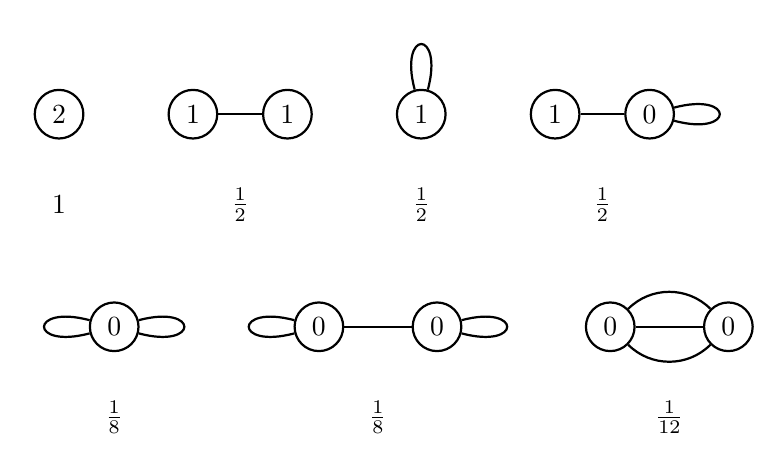
\begin{tikzpicture}[scale=1,transform shape,every loop/.style={min distance=8mm,looseness=10}]
        \node[circle,draw=black,thick] (a) at (0,0) {$2$};
        \node at (0,-1.15) {$1$};

        \node[circle,draw=black,thick] (b1) at (1.7,0) {$1$};
        \node[circle,draw=black,thick] (b2) at (2.9,0) {$1$};
        \draw[thick] (b1) -- (b2);
        \node at (2.3,-1.15) {$\frac{1}{2}$};

        \node[circle,draw=black,thick] (c) at (4.6,0) {$1$};
        \draw[thick] (c) edge[loop above] (c);
        \node at (4.6,-1.15) {$\frac{1}{2}$};

        \node[circle,draw=black,thick] (d1) at (6.3,0) {$1$};
        \node[circle,draw=black,thick] (d2) at (7.5,0) {$0$};
        \draw[thick] (d1) -- (d2);
        \draw[thick] (d2) edge[loop right] (d2);
        \node at (6.9,-1.15) {$\frac{1}{2}$};

        \node[circle,draw=black,thick] (e) at (0.7,-2.7) {$0$};
        \draw[thick] (e) edge[loop left] (e);
        \draw[thick] (e) edge[loop right] (e);
        \node at (0.7,-3.85) {$\frac{1}{8}$};

        \node[circle,draw=black,thick] (f1) at (3.3,-2.7) {$0$};
        \node[circle,draw=black,thick] (f2) at (4.8,-2.7) {$0$};
        \draw[thick] (f1) -- (f2);
        \draw[thick] (f1) edge[loop left] (f1);
        \draw[thick] (f2) edge[loop right] (f2);
        \node at (4.05,-3.85) {$\frac{1}{8}$};

        \node[circle,draw=black,thick] (g1) at (7.0,-2.7) {$0$};
        \node[circle,draw=black,thick] (g2) at (8.5,-2.7) {$0$};
        \draw[thick] (g1) -- (g2);
        \draw[thick] (g1) to[bend left=45] (g2);
        \draw[thick] (g1) to[bend right=45] (g2);
        \node at (7.75,-3.85) {$\frac{1}{12}$};
    \end{tikzpicture}
    \caption{亏格二无腿的七张稳定图，按顶点亏格标记并以 \(\frac{1}{\ab|\Aut\Gamma|}\) 加权。幻灯片上每个顶点画成其黎曼面分支。}%
    \label{fig:g2stable}
\end{figure}

\begin{rmk}
    这些是稳定曲线的对偶图，不是~\Cref{fig:tropgraphs} 中的图，后者是对 log GLSM 约化理论应用热带分解公式得到的刚性热带型。两种拓扑列表在此恰好重合，但顶点含义不同。这里它是带拓扑场论张量的定义域曲线的分支。那里它是二部热带曲线的层，带有 log 或 \(\infty\)-顶点模问题。
\end{rmk}

对形式路线，我们内在地定义归一化势
\[ P_2^{\lambda} \coloneqq \frac{Y}{I_0^2}F_2^{\lambda}, \qquad Y = L^5. \]
完整图求和落在 \(\Q[L,\mc{X}_1,\mc{X}_2,\mc{X}_3,\mc{Y}_1]\) 中，等于
\begin{align*}
    P_2^{\lambda} ={}& -\frac{1}{128}L^{12} - \frac{23}{960}L^8\mc{X}_1 - \frac{9}{640}L^8\mc{Y}_1 + \frac{109}{16000}L^7 \\
    &- \frac{3}{80}L^4\mc{X}_1^2 - \frac{19}{320}L^4\mc{X}_1\mc{Y}_1 - \frac{3}{80}L^4\mc{Y}_1^2 - \frac{1}{64}L^4\mc{X}_2 \\
    &+ \frac{19}{1920}L^3\mc{X}_1 - \frac{47}{48000}L^2 \\
    &- \frac{67}{1152}\mc{X}_1^3 - \frac{101}{1152}\mc{X}_1^2\mc{Y}_1 - \frac{5}{48}\mc{X}_1\mc{Y}_1^2 - \frac{1}{24}\mc{Y}_1^3 \\
    &- \frac{25}{288}\mc{X}_1\mc{X}_2 - \frac{1}{48}\mc{X}_2\mc{Y}_1 - \frac{19}{1152}\mc{X}_3.
\end{align*}
为清楚起见，这是精确的形式 \(\lambda\)-扭曲答案，不是 \(F_2^{\mr{GW}}\)。还注意 \(Y = L^5\) 是判别式生成元，而 \(\mc{Y}_1\) 是对数导数生成元。

\subsection{有限生成与扩张族}%
\label{sub:Finite generation and the extended family}

回顾上面的有限生成环 \(\mc{R} = \Q[A,B_1,B_2,B_3,Y]\)，我们按如下分级：
\[ \deg A = \deg B_1 = 1, \qquad \deg B_2 = 2, \qquad \deg B_3 = 3, \qquad \deg Y = 0. \]
对如前的 \(\phi_k = I_{1,1}\cdots I_{k,k}H^k\)，设
\[ \wt{\Omega}^{\lambda}_{g,n} \coloneqq 5^{g-1}\ab(\frac{Y}{I_0^2})^{g-1}\Omega^{\lambda,\tau}_{g,n}. \]

\begin{thm}[Graded finite generation {\cite{GJRstructure}}]%
\label{thm:graded finite generation}
    我们有
    \[ \wt{\Omega}^{\lambda}_{g,n}(\phi_{a_1}, \ldots, \phi_{a_n}) \in \bigoplus_{k \geq 0}\lambda^{5k}H^{2(3g-3+\sum_i a_i - 5k)}(\Mbar_{g,n},\Q)\otimes \mc{R}_{3g-3+\sum_i a_i}. \]
    因而在组装二部剩余图后，扩张族的非等变分支满足
    \[ P^{\mbf{C}}_{g,n} = 5^{1-g}\int_{\Mbar_{g,n}}\wt{\Omega}^{\mbf{C}}_{g,n}(\phi_1^{\otimes n}) = \ab( \frac{Y}{I_0^2})^{g-1}\int_{\Mbar_{g,n}}\Omega^{\mbf{C}}_{g,n}(\phi_1^{\otimes n}) \in \mc{R}_{3g-3+n}. \]
\end{thm}

特别地，在每个固定的 \((g,n)\) 只有有限多个分级单项式可出现，只有 \(3g-3+n\) 阶以内的 \(R\)-矩阵有贡献。

我们用二部图求和组织扩张理论：
\[ \Omega^{\mbf{C},\lambda}_{g,n} = \sum_{\Gamma \text{ bipartite}} \frac{1}{\ab|\Aut\Gamma|}\prod_{v\in V_{\infty}(\Gamma)} C^{\infty}_{g_v,\mu_v}(\mbf{C};\vec{a}_v) \prod_{v \in V_0(\Gamma)}C^{\lambda}_{g_v,\vec{\delta}_v}(\vec{a}_v)\prod_{e \in E(\Gamma)}V_e, \]
其中 \(C^{\infty}\) 是有效或亚纯顶点因子，\(C^{\lambda}\) 是形式零顶点关联函数，\(\mu_v\) 与 \(\vec{\delta}_v\) 记录关联次数，\(V_e\) 是边因子。极限 \(\lambda \to 0\) 只在完整图求和后取。设 \(\mbf{C}=0\) 留下形式 \(\lambda\)-扭曲首部。设 \(\mbf{C}=\mbf{C}^{\mr{eff}}\) 并令 \(\lambda\to0\) 回到五次三维流形的 Gromov-Witten 理论。微分一条通用边即切断它，给出全纯反常方程，而有效顶点不受影响。

为推导全纯反常方程，记 \(P^{\mbf{C}}_g \coloneqq P^{\mbf{C}}_{g,0}\) 并引入
\[ \mc{U} = B_1, \qquad \mc{V} = A + 2B_1, \qquad \mc{V}_2 = D\mc{U} + \mc{U}^2 - \mc{U}\mc{V}, \qquad \mc{V}_3 = (D+\mc{V})\mc{V}_2, \]
以及两个非全纯方向
\[ \partial_1 = \partial_{\mc{U}}, \qquad \partial_0 = \partial_{\mc{V}} - \mc{U}\partial_{\mc{V}_2} - \mc{U}^2\partial_{\mc{V}_3}. \]

\begin{thm}[Holomorphic anomaly equation for the extended family {\cite{GJRstructure}}]
    我们有
    \[ -\partial_0 P^{\mbf{C}}_g = \frac{1}{2}P^{\mbf{C}}_{g-1,2} + \frac{1}{2}\sum_{\substack{g_1+g_2=g\\g_1,g_2\geq1}}P^{\mbf{C}}_{g_1,1}P^{\mbf{C}}_{g_2,1}, \qquad -\partial_1 P^{\mbf{C}}_g = 0. \]
\end{thm}

我们用~\Cref{sub:The holomorphic anomaly equation} 的切割论证证明它，之所以可行是因为 \(R\)-矩阵传播子的导数恰为
\[ 5\mc{B}_{\partial_0} = \bar{\phi}_1 \otimes \bar{\phi}_1, \qquad 5\mc{B}_{\partial_1} = \bar{\phi}_0\otimes\bar{\phi}_2 + \bar{\phi}_2\otimes\bar{\phi}_0. \]
\(R^{-1}\) 与每条边的导数仍留在同一分级环中，所以切断一条微分过的边在 \(\mc{R}\) 中闭合为低亏格关联函数。若设 \(\mbf{C}=0\)，则回到形式 \(\lambda\)-扭曲理论的同样方程。

\subsection{边界条件}%
\label{sub:Boundary conditions}

我们将用两类条件约束全纯不确定性。

第一，我们用 orbifold 或 Landau-Ginzburg 点 \(q = \infty\)，等价地 \(L \to 0\) 处的正则性。对形式或组装后的扩张势 \(F_g^{\star}\)，设
\[ \mc{P}_g^{\mr{orb},\star} \coloneqq \ab(\frac{L}{I_0})^{2g-2}F_g^{\star} = \Phi_g^{\star}(\mc{X}_1,\mc{X}_2,\mc{X}_3,\mc{Y}_1,L^{-1},L^5). \]
\Cref{thm:graded finite generation} 界定了 \(L\) 可能的 Laurent 幂次，而形式 LG/CY 对应说，在解析延拓并等同归一化的 CY 基与 LG 基后，同一个形式 \(R\)-矩阵多项式描述两相。因此
\[ \lim_{L\to0}\Phi_g^{\star}(\mc{X}_1,\mc{X}_2,\mc{X}_3,\mc{Y}_1,L^{-1},L^5) \text{ 存在}, \]
而对 \(f_g(Y) = \sum_{i=0}^{3g-3}a_{i,g}Y^i\)（其中 \(Y = L^5\)）五次三维流形的界为
\[ a_{i,g} = 0 \qquad \text{当 } i \leq \ceil*{\frac{3(g-1)}{5}} \text{ 时}. \]
注意这是关于组装后的归一化图贡献的断言，不是关于单个裸亚纯或 rubber 顶点关联函数的。

第二，我们研究 conifold。设
\[ q = 5^{-5}(1+t_c)^{-1}, \qquad T_c = \frac{I_1^{\mr{co}}(t_c)}{I_0^{\mr{co}}(t_c)}, \]
其中 \(I_0^{\mr{co}}, I_1^{\mr{co}}\) 组成局部 conifold 周期对，归一化使消失的平坦坐标在 conifold 处满足 \(T_c = 0\)。给定有限生成数据中的有理表达式 \(f\)，把所有生成元的 Laurent 展开代入为 \(T_c\) 的级数，即得其 conifold 值 \(f^{\mr{co}}\)。\Cref{thm:graded finite generation} 给出极点界
\[ F_g^{\mbf{C},\mr{co}} = O\ab(T_c^{-(2g-2)}), \]
但我们需要的是更强的\textit{间隙}条件
\[ F_g^{\mr{co}} = \frac{c_g}{T_c^{2g-2}} + O(1), \]
即每个中间负幂 \(T_c^{-(2g-3)}, \ldots, T_c^{-1}\) 都消失。这是 \(2g-2\) 个条件，不是有限生成蕴含的。

\begin{conj}[Formal conifold gap]%
\label{conj:formal conifold gap}
    形式 \(\lambda\)-扭曲势有通用首项
    \[ F_g^{\lambda,\mr{co}} = \frac{(-1)^{g-1}B_{2g}}{2g(2g-2)T_c^{2g-2}} + O(1), \]
    其中 \(B_{2g}\) 是 Bernoulli 数。
\end{conj}

\begin{exm}
    在亏格二算得的展开开头为
    \[ F_2^{\lambda,\mr{co}} = \frac{1}{240T_c^2} + \frac{31}{6000} - \frac{7169}{3600000}T_c + \frac{22951}{45000000}T_c^2 + O(T_c^3). \]
    这是亏格二间隙，而不仅是极点阶界。
\end{exm}

我们还须考虑剩余图中出现的形式关联函数带的有理后代插入，即
\[ C^{\lambda}_{g,\vec{\delta}}(\vec{a}) \coloneqq \ab< \frac{H^{3-a_1}}{-5H\ab(-\frac{5H}{\delta_1}-\psi_1)}, \ldots, \frac{H^{3-a_n}}{-5H\ab(-\frac{5H}{\delta_n}-\psi_n)}>^{\lambda}_{g,n} \]
其中 \(\delta_i \geq 1\) 且 \(a_i \in \ab\{0,1,2,3,4\}\)。

\begin{conj}[Regularity with special insertions]%
\label{conj:special correlator regularity}
    我们有 \(\ab(C^{\lambda}_{g,\vec{\delta}}(\vec{a}))^{\mr{co}} = O(1)\)。
\end{conj}

对固定的 \(\vec{a}\) 与 \(\vec{\delta}\)，\(\psi\)-展开的单项可能有极点。注意断言关乎完整的有理后代插入，其负幂在对 \(\vec{a}\) 取剩余图求和之前相消。它是关于这些特定形式关联函数的断言，而不是关于每个未组装亚纯关联函数的。

我们可用~\Cref{conj:formal conifold gap,conj:special correlator regularity} 把间隙传到五次三维流形的 Gromov-Witten 理论。剩余图贡献形如
\[ \sum_{\vec{a}} \prod_{v \in V_{\infty}(\Gamma)}I_0^{2g_v-2+\ell(\mu_v)}C^{\infty}_{g_v,\mu_v}(\vec{a}_v)\prod_{v\in V_0(\Gamma)}C^{\lambda}_{g_v,\vec{\delta}_v}(\vec{a}_v), \]
而 \(C^{\infty}\) 因子是 \(q\) 的有限多项式，所以在 conifold 处正则。于是形式首部间隙连同特殊关联函数的正则性蕴含扩张族的间隙，从而给出五次三维流形的间隙。

\begin{rmk}
    \Cref{conj:formal conifold gap,conj:special correlator regularity} 在一般情形是公开的，但 Guo-Janda-Ruan 已对五次三维流形验证到 \(g \leq 5\)。扩张族的极点界是定理，间隙由两个猜想推出，并由显式计算对 \(g \leq 5\) 证明。在这些讲座时，五次三维流形 Gromov--Witten 理论的全亏格间隙因此以它们为条件，在 \(g \leq 5\) 时无条件成立。\footnote{随后，Chang--Guo--You--Zhang 在~\cite{CGYZ2026} 中宣布了五次三维流形 Gromov--Witten 理论 conifold 间隙的全亏格证明。上面的两个形式理论猜想是独立的陈述。}
\end{rmk}

把所有这些放在一起，我们从 Picard-Fuchs 数据出发，计算 Givental \(R\)-矩阵与算子 \(S_{\tau}(z)\)。然后得到形式稳定图与亚纯剩余图，用全纯反常方程与有限生成，最后施加 orbifold 与 conifold 边界条件以确定 \(F_g^{\mr{GW}}\)。
